%%%%%%%%%%%%%%%%%%%%%%%%%%%%%%%%%%%%%%%%%%%%%%%%%%%%%%%%%%%%%%%%%%%%%%%%%%%%%
%
%  System        : 
%  Module        : 
%  Object Name   : $RCSfile$
%  Revision      : $Revision$
%  Date          : $Date$
%  Author        : $Author$
%  Created By    : Robert Heller
%  Created       : Mon Jul 15 17:34:14 2019
%  Last Modified : <190727.2307>
%
%  Description 
%
%  Notes
%
%  History
% 
%%%%%%%%%%%%%%%%%%%%%%%%%%%%%%%%%%%%%%%%%%%%%%%%%%%%%%%%%%%%%%%%%%%%%%%%%%%%%
%
%    Copyright (C) 2019  Robert Heller D/B/A Deepwoods Software
%			51 Locke Hill Road
%			Wendell, MA 01379-9728
%
%    This program is free software; you can redistribute it and/or modify
%    it under the terms of the GNU General Public License as published by
%    the Free Software Foundation; either version 2 of the License, or
%    (at your option) any later version.
%
%    This program is distributed in the hope that it will be useful,
%    but WITHOUT ANY WARRANTY; without even the implied warranty of
%    MERCHANTABILITY or FITNESS FOR A PARTICULAR PURPOSE.  See the
%    GNU General Public License for more details.
%
%    You should have received a copy of the GNU General Public License
%    along with this program; if not, write to the Free Software
%    Foundation, Inc., 675 Mass Ave, Cambridge, MA 02139, USA.
%
% 
%
%%%%%%%%%%%%%%%%%%%%%%%%%%%%%%%%%%%%%%%%%%%%%%%%%%%%%%%%%%%%%%%%%%%%%%%%%%%%%

\chapter{LCCCANCape: LCC CAN Tranceiver Cape}

\section{GPIO Pins Used and stacking restrictions.}

This board uses two pins on header P9: 24 and 26 in pin mux mode2, which makes 
pin 24 Can1 RX, and pin 26 Can1 TX.  Only one of these capes can be on any 
Beagle Bone Black.


\section{Circuit Description}

\begin{figure}[hbpt]\begin{centering}%                                         
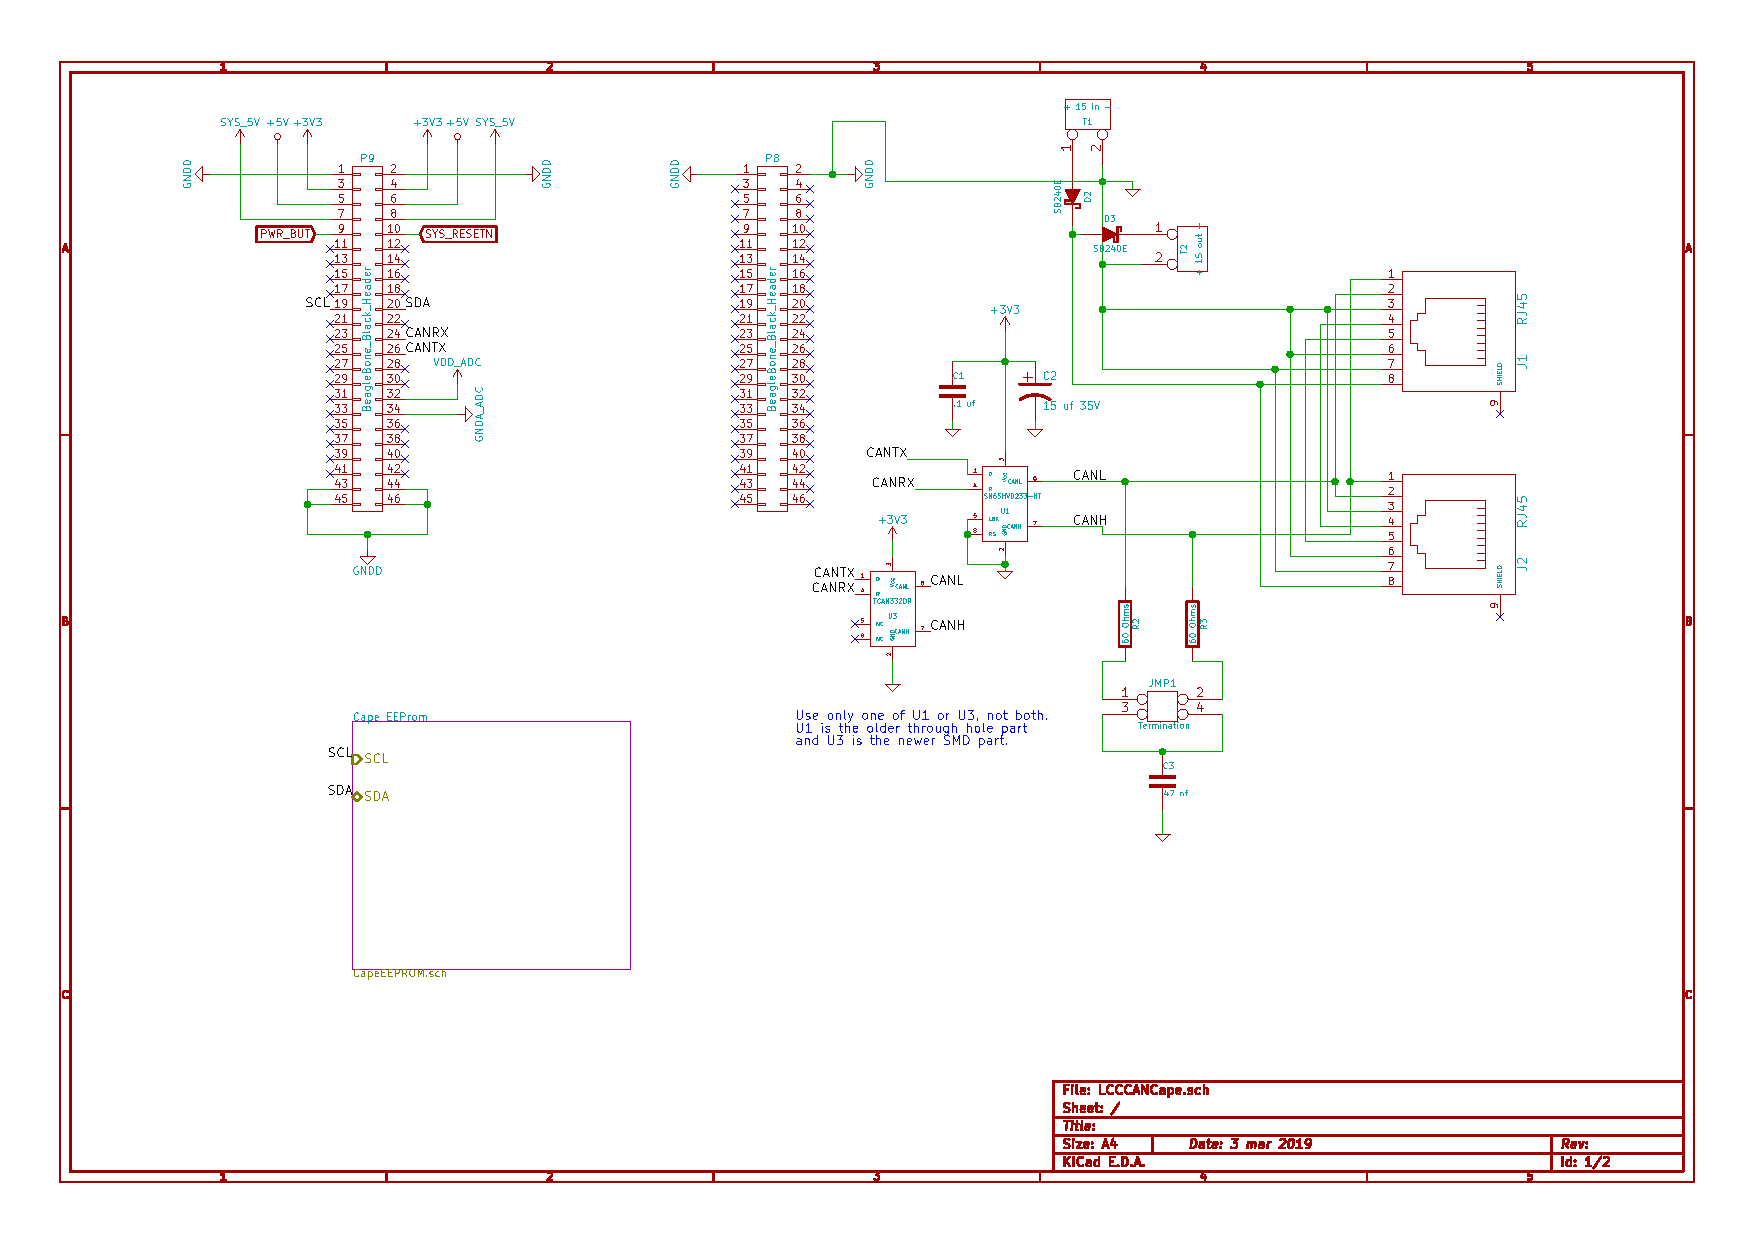
\includegraphics[width=5in]{LCCCANCape-1.pdf}                               
\caption{Circuit Diagram of the LCCCANCape}                               
\end{centering}\end{figure}                                                    
This circuit contains two sectins.  There is the transciever section, which 
includes the transciver itself, the termination block, the two RJ45 jacks, and 
two terminal blocks for injecting and tapping into the power carried in the 
CAT 5 cable.  Power is not used to power the Beagle Bone Black.  The other 
section is the Cape EErom circuit.  The Cape EEProm contains         
information about the cape and the name and version of the overlay that needs  
to be loaded by uBoot.  

\section{Parts List}

\section{Circuit Board Layout}

\section{Downloadables and Software Support}

